\documentclass[8pt,xcolor=table,dvipsnames]{beamer}
\usepackage{pgfpages}
\usepackage{yhmath}
\newcommand{\Mod}[1]{\ (\mathrm{mod}\ #1)}
\providecommand{\half}{\frac{1}{2}}
\newcommand{\dg}{^\circ}
\newcommand{\arc}[1]{\wideparen{#1}}
\usetheme{Madrid}

\title{Geometric Transformations IV}
\subtitle{UMC K1, 2024}
\author{Nghia Doan}
\institute{MCC Club \& Competitions}
\date{\today}

\begin{document}

\section{Homothety}

\begin{frame}[t]
    \frametitle{Geometric Transformations IV}
    \framesubtitle{Homothety - Definition}
    A \textbf{homothety} (or homothecy) is a transformation of space
    which dilates distances \textit{with respect to a fixed point.}

    \bigbreak
    A homothety can be an \textit{enlargement} (resulting figure is larger),
    \textit{identity} transformation (resulting figure is congruent),
    or a \textit{contraction} (resulting figure is smaller).

    \bigbreak
    A homothety with center $O$ and factor $k$ sends point $A$ to a point $A'$, and
    \[
        OA'= k\cdot OA.
    \]
    \begin{center}
        \includegraphics[width=6cm]{../Learning-Problem-Solving-2nd-Edition/asy/pdf/homothety-1.pdf}
    \end{center}
    This is denoted by $\mathcal{H}_{(O, k)}$.
\end{frame}

\begin{frame}[t]
    \frametitle{Geometric Transformations IV}
    \framesubtitle{Homothety - Image Types}
    \begin{overprint}
        \onslide<1>Let $\mathcal{H}_{(O, k)}$ be a homothety.
        For point $A$, $\mathcal{H}_{(O, k)}(A) = A' \Rightarrow O,A,A'$ colliner.
        Thus, the lines connecting each point of a polygon  to its corresponding point of a homothetic polygon
        are all concurrent.
        \begin{center}
            \includegraphics[width=5cm]{../Learning-Problem-Solving-2nd-Edition/asy/pdf/homothety-1.pdf}
        \end{center}
        For line $XY$, $\mathcal{H}_{(P, k)}(AB) = A'B' \Rightarrow AB \parallel A'B'.$

        For $\triangle ABC$, $\mathcal{H}_{(A, k)}(\triangle ABC) = \triangle AB'C' \Rightarrow \triangle ABC \sim \triangle AB'C'.$

        The resulting image of a circle from a homothety is also a circle.
        \begin{center}
            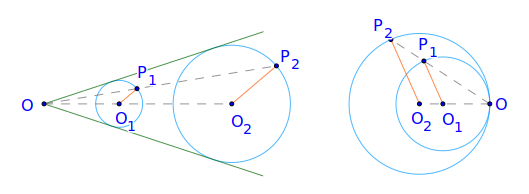
\includegraphics[width=7cm]{./svg/pdf/homothety-circles.pdf}
        \end{center}
    \end{overprint}
\end{frame}

\begin{frame}[t]
    \frametitle{Geometric Transformations IV}
    \framesubtitle{Homothety - Factor}
    \begin{overprint}
        \onslide<1>Let $\mathcal{H}_{(S, k)}$ be a homothety.
        \bigbreak
        If $k > 0$, then the image and the original will be on the same side of the center,
        they are are scaled and translated similar to one another.
        \begin{center}
            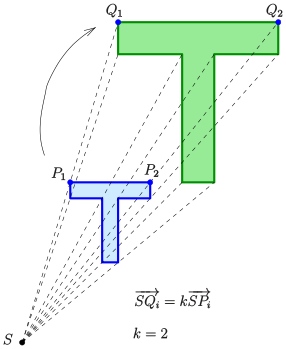
\includegraphics[width=4cm]{./svg/pdf/Zentr-streck-T-e.pdf}
            \qquad
            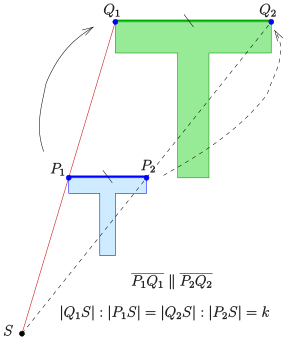
\includegraphics[width=4cm]{./svg/pdf/Zentr-streck-T-S-e.pdf}
        \end{center}
        If $|k| > 1$, then the homothety is a magnification (enlargement);
        If $|k| < 1$, then it is a reduction (shrinking).
        \onslide<2>Let $\mathcal{H}_{(S, k)}$ be a homothety.
        \bigbreak
        If $k < 0$, the image and the original will be on different sides of the center,
        i.e. the center will be between them. 
        A homothety with factor $k=-1$ is a $180^\circ$ rotation about the center.
        \begin{center}
            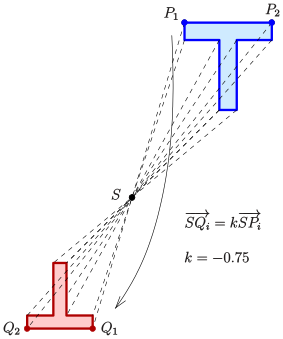
\includegraphics[width=4cm]{./svg/pdf/Zentr-streck-T-nk-e.pdf}
        \end{center}
        \onslide<3>Circles are geometrically similar to one another and \textit{rotation invariant}.
        These two homothetic centers lie on the line joining the centers of the two given circles.
        \begin{center}
            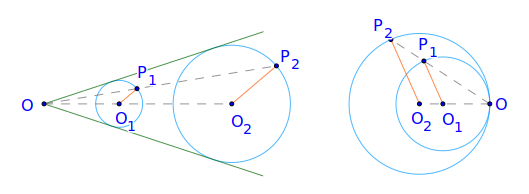
\includegraphics[width=6cm]{./svg/pdf/homothety-circles.pdf}
            \includegraphics[width=6cm]{../Learning-Problem-Solving-2nd-Edition/asy/pdf/homothety-2.pdf}
        \end{center}
        The common external tangents pass through the external homothetic center,
        while the common internal tangents pass through the internal homothetic center.
        \bigbreak
        If the circles have the same radius (but different centers), they have no external homothetic center.
        If the circles have the same center, they have only one homothetic center and that is the common center of the circles.
    \end{overprint}
\end{frame}

\begin{frame}[t]
    \frametitle{Geometric Transformations IV}
    \framesubtitle{Homothety - Factor}
    Let $\mathcal{H}_{3\ (S_3,k_3)}$ be the compositions of $\mathcal{H}_{1\ (S_1,k_1)}$
    and $\mathcal{H}_{2\ (S_2,k_2)}$ (below on the left): 
    \[
        \mathcal{H}_{3\ (S_3,k_3)} = \mathcal{H}_{2\ (S_2,k_2)} \circ \mathcal{H}_{1\ (S_1,k_1)}
        \Rightarrow S_3 \in S_1S_2,\ k_3=k_1 \cdot k_2.
    \]
    \begin{center}
        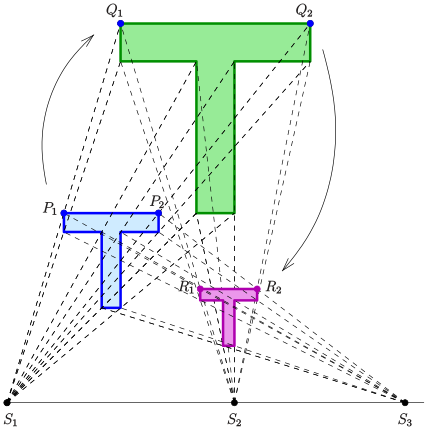
\includegraphics[width=4cm]{./svg/pdf/Zentr-streck-TT-e.pdf}
        \qquad \qquad
        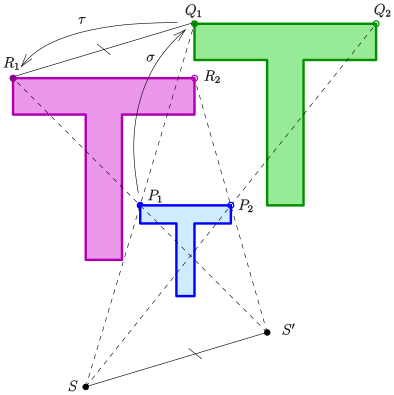
\includegraphics[width=4cm]{./svg/pdf/Zentr-streck-T-st-e.pdf}
    \end{center}
    The composition of a homothety and a translation is a homothety (above on the right).
\end{frame}

\section{Homothety - Examples}

\begin{frame}[t]
    \frametitle{Geometric Transformations IV}
    \framesubtitle{Homothety - Example 1}
    \begin{example}
        Circles $\omega_1$ and $\omega_2$ are tangent at $M$.
        A line through $M$ intersects $\omega_1$ and $\omega_2$ at $A_1$ and $A_2.$
        Show that the tangent lines to $\omega_1$ at $A_1$ and to $\omega_2$ at $A_2$ are parallel.
    \end{example}
    \onslide<2>Consider the homothety $\mathcal{H}(M,\pm\frac{r_2}{r_1})$, where $r_1$, $r_2$ are the radii of circles $\omega_1$, $\omega_2$ respectively,
    and \textit{the minus sign is chosen in the case of exterior tangency} of the two circles (on the left),
    while \textit{the plus sign is chosen in the case of interior tangency} of the two circles (on the right).
    \begin{center}
        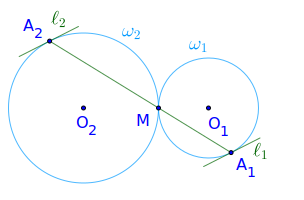
\includegraphics[width=3.5cm]{./svg/pdf/homothety-p1.pdf}
        \qquad
        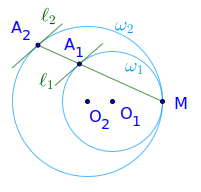
\includegraphics[width=2.4cm]{./svg/pdf/homothety-p1b.pdf}
    \end{center}
    This transformation carries the circle $\omega_1$ of radius $r_1$ into a circle of radius $r_2$, tangent to $\omega_1$ at the point $M$;
    that is, it carries $\omega_1$ into $\omega_2$.

    The point $A_1$ on the circle $\omega_1$ is carried by this transformation into the point $A_2$ on the circle $\omega_2$,
    and the tangent line $\ell_1$ to $\omega_1$ at $A_1$ is carried into the tangent line $\ell_2$ to $\omega_2$ at $A_2.$
    
    Since \textbf{the line $\ell_2$ is obtained from $\ell_1$ by a homothety, the two lines are parallel}.
\end{frame}

\begin{frame}[t]
    \frametitle{Geometric Transformations IV}
    \framesubtitle{Homothety - Example 2}
    \begin{example}
        Let $\omega_1$ and $\omega_2$ be two disjoint circles, neither inside the other.
        Let $m$ be a common tangent to $\omega_1$ and $\omega_2$ and assume that $\omega_1$ and $\omega_2$ are both on the same side of $m$.
        Let $n$ be another common tangent, with $\omega_1$ and $\omega_2$ both on the same side of $n$.
        Let $M$ be the point of intersection of $m$ and $n$. Let $\ell$ be a line through $M$ meeting $\omega_1$ in points $A$ and $B$ and meeting $\omega_2$ in points $C$ and $D$.
        Finally, let $E$ be the point of tangency of $m$ and $\omega_1$ and let $F$ be the point of tangency of $m$ and $\omega_2$.
        Prove that:
        \begin{enumerate}
            \item $\triangle ABE \sim \triangle CDF$.
            \item $[ABE]/[CDF] = (r_1/r_2)^2,$ where $r_1$ and $r_2$ are the radii of circles $\omega_1$ and $\omega_2$, respectively.
            \item $M$ is on the line through the centroids (intersection of the medians) of $\triangle ABE$ and $\triangle CDF$.
        \end{enumerate}
    \end{example}
    \begin{center}
        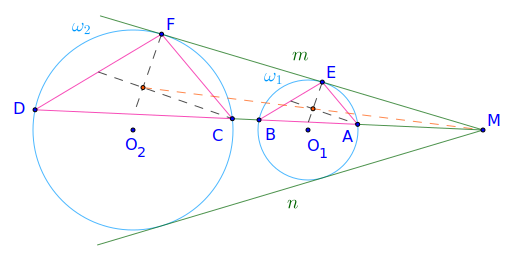
\includegraphics[width=6cm]{./svg/pdf/homothety-p2.pdf}
    \end{center}
\end{frame}

\begin{frame}[t]
    \frametitle{Geometric Transformations IV}
    \framesubtitle{Homothety - Example 2}
    Consider the homothety with center $M$ and coefficient $k = r_2/r_1$.
    This transformation carries the lines $m$ and $n$ onto themselves, and carries the circle $\omega_1$ tangent to $m$ and $n$ and with radius $r_1$ onto
    a circle tangent to $m$ and $n$ and with radius $r_2$; that is, it carries $\omega_1$ onto $\omega_2$.    
    \begin{center}
        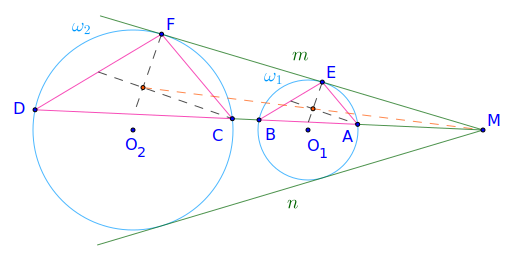
\includegraphics[width=6cm]{./svg/pdf/homothety-p2.pdf}
    \end{center}
    Also, the line $\ell$ is carried into itself, the segment $AB$ is carried into $CD$, the point $E$ into $F$ and,
    consequently, \textbf{triangle $ABE$ is carried onto triangle $CDF$}.
    From this it follows that these triangles are similar, and that the \textbf{similarity coefficient is $k = r_2/r_1$}; therefore $[ABE]/[CDF] = (r_1/r_2)^2.$

    \bigbreak
    Finally, from the fact that triangle $CDF$ is obtained from triangle $ABE$ by a homothety with center $M$,
    it follows that \textbf{the line joining two corresponding points} of these triangles,
    for example, their centroids (the points of intersection of their medians),
    \textbf{passes through the point $M$}. 
\end{frame}

\begin{frame}[t]
    \frametitle{Geometric Transformations IV}
    \framesubtitle{Homothety - Example 3}
    \begin{example}
        Prove that the line joining the midpoints of the two parallel sides of a trapezoid passes through the point of intersection of the extensions of the other two sides,
        as well as through the point of intersection of the diagonals.
    \end{example}
    \begin{center}
        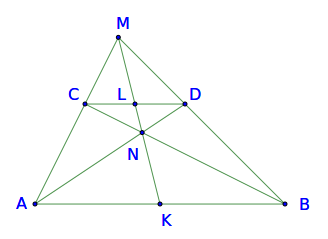
\includegraphics[width=3.5cm]{./svg/pdf/homothety-p3b.pdf}
    \end{center}
    \onslide<2->The homothety with center at the point $M$ of intersection of the extensions of sides $AC$ and $BD$ of trapezoid $ABDC$
    and with coefficient $CD/AB$ carries the segment $AB$ onto the segment $CD$ and carries the midpoint $K$ of $AB$ into the midpoint $L$ of side $CD$
    Therefore, the line $KL$ passes through the homothety center $M$.

    \onslide<3>The point $K$ is also carried onto the point $L$ by the homothety with center at the point $N$ of intersection of the diagonals $AD$ and $BC$ of the trapezoid
    and with the (negative) coefficient $-CD/AB$. This transformation carries the segment $AB$ onto $CD$. Therefore the line $KL$ also passes through
    the point $N.$

    \onslide<4>\textbf{Is this true for non-parallelogram convex quadrilateral?} 
\end{frame}

\begin{frame}[t]
    \frametitle{Geometric Transformations IV}
    \framesubtitle{Homothety - Example 4}
    \begin{overprint}
        \onslide<1>
        \begin{example}
            Three concentric circles $\omega_1$, $\omega_2$, and $\omega_3$ are given.
            \bigbreak
            Draw a line $\ell$ meeting $\omega_1$, $\omega_2$, and $\omega_3$ in order in points $A$, $B$, and $C$ such that $AB = BC.$
        \end{example}
        \begin{center}
            \includegraphics[width=5cm]{./svg/pdf/homothety-p4a.pdf}
        \end{center}
        \onslide<2>We first solve a problem with two concentric circles.
        Assume that $AB'=B'C.$ Let $O'$ be the midpoint of $AO.$

        \bigbreak
        Then the homothety centred at $A$ with similarity coefficient 2 brings $B'$ to $C'$ and $O'$ to $O.$
        Thus it brings a circle centred at $O'$ (with the radius equal to half of the radius of $\omega_3$) to the circle $\omega_3$.
        \begin{center}
            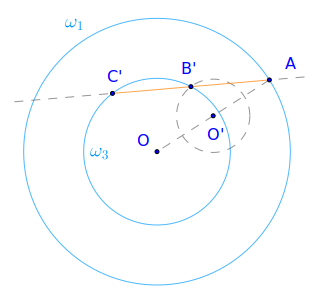
\includegraphics[width=5cm]{./svg/pdf/homothety-p4b.pdf}
        \end{center}
        \onslide<3>Now, the homothety centred at $A$ with similarity coefficient 2 brings $O'$ to $O$, circle $(O')$ to $\omega_3$.

        \bigbreak
        Thus it brings $B$ - the intersection of $(O')$ with $\omega_2$ - to $C$ - point on $\omega_3$.
        Because of the similarity coefficient: $AB=BC.$
        \begin{center}
            \includegraphics[width=5cm]{./svg/pdf/homothety-p4c.pdf}
        \end{center}

        \textbf{How about $A, B, C, D$ on four concentric circles such that $AB=CD$?} 
    \end{overprint}
\end{frame}

\begin{frame}[t]
    \frametitle{Geometric Transformations IV}
    \framesubtitle{Homothety - Example 5}
    \begin{overprint}
        \onslide<1>
        \begin{example}
            Let a “hinged” parallelogram A BCD be given. More precisely, the lengths of the sides are fixed, and vertices $A$ and $B$ are fixed, but vertices $C$ and $D$ are movable.
            \bigbreak
            As $C$ and $D$ move, what is the locus of point $Q$, the intersection of the diagonals?
        \end{example}
        \begin{center}
            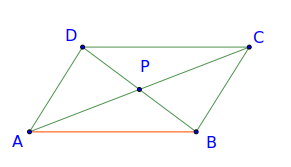
\includegraphics[width=5cm]{./svg/pdf/homothety-p5a.pdf}
        \end{center}
        \onslide<2>Since side $BC$ does not change in length and $B$ is fixed, $C$ moves on a circle with center $B$ as the “hinged” parallelogram moves.
        But $Q$ is obtained from $C$ by a central similarity transformation with center at the fixed point $A$ and with coefficient $1/2$.
        Therefore $Q$ moves on the circle $\gamma$ obtained by this transformation (centred at $F$ midpoint of $AB$ with radius $r$ half of $BC$)
        from the circle $\omega$ on which $C$ moves.
        \begin{center}
            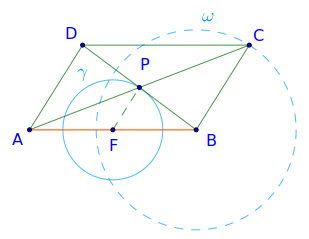
\includegraphics[width=5cm]{./svg/pdf/homothety-p5b.pdf}
        \end{center}
        \textbf{Is this true for arbitrary convex quadrilateral?} 
    \end{overprint}
\end{frame}

\begin{frame}[t]
    \frametitle{Geometric Transformations IV}
    \framesubtitle{Diameter of the Incirle}
    \begin{example}
        Let the incircle of triangle $ABC$ touch side $BC$ at $D$, and let $DE$ be a diameter of the circle.
        If line $AE$ meets $BC$ at $F$, then $BD = CF$
    \end{example}
    \begin{overprint}
        \onslide<1>\begin{center}
            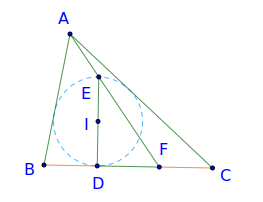
\includegraphics[width=4cm]{./svg/pdf/diameter-incircle-1.pdf}
        \end{center}
        \onslide<2>The homothety with center $A$ that carries the incircle to an excircle (why?).

        The diameter $DE$ of the incircle is mapped to the diameter of the excircle perpendicular to $BC$.

        It follows that $E$ must get mapped to the point of tangency between the excircle and $BC$.
        Since the image of $E$ must lie on the line $AE$, it must be $F$.

        That is, the excircle is tangent to $BC$ at $F.$ Then, it follows easily that $BD=CF$ (how?).
        \begin{center}
            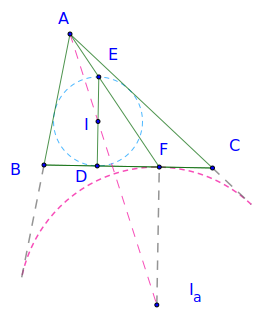
\includegraphics[width=3.5cm]{./svg/pdf/diameter-incircle-2.pdf}
        \end{center}
    \end{overprint}
\end{frame}

\begin{frame}[t]
    \frametitle{Geometric Transformations IV}
    \framesubtitle{Nine point circle}
    \begin{example}
        For a given triangle, prove that there exists a circle, which passes through:
        (i) the three feet of the altitudes, (ii) the three midpoints of the sides,
        and (iii) the three midpoints of the segments joining the vertices of the triangle to its orthocenter.
    \end{example}
    \begin{center}
        \includegraphics[width=5cm]{../Learning-Problem-Solving-2nd-Edition/asy/pdf/nine-points-circle-1.pdf}
    \end{center}
\end{frame}

\begin{frame}[t]
    \frametitle{Geometric Transformations IV}
    \framesubtitle{Nine point circle}
    \begin{overprint}
        \onslide<1>First, $E_a$, $E_b$, and $E_c$ are midpoints of $HA$, $HB$, and $HC$.
        \onslide<2>Second, if $X_a$, $X_b$, and $X_c$ be the intersection of $AH_a$, $BH_b$, and $CH_c$ with the circle $(ABC)$,
        then $HH_a=H_aX_a$, $HH_b=H_bX_b$, and $HH_c=H_cX_c$.
        \onslide<3>Third, if $Y_a$, $Y_b$, and $Y_c$ be points such that $AHBY_c$, $BHY_a$, and $CHAY_b$ are parallelograms,
        then $Y_a$, $Y_b$, and $Y_c$ are on the circle $(ABC)$ (because for example $ACBY_a$ is cyclic)
        \onslide<4>Therefore the homothety centred at $H$ with factor 2 maps
        $E_a$, $E_b$, and $E_c$ to $A$, $B$, and $C$;
        $H_a$, $H_b$, and $H_c$ to $X_a$, $X_b$, and $X_c$;
        and $M_a$, $M_b$, and $M_c$ to $Y_a$, $Y_b$, and $Y_c$.
        \bigbreak
        Hence, all nine points are on the circle $\omega.$
    \end{overprint}
    \begin{center}
        \includegraphics[width=5cm]{../Learning-Problem-Solving-2nd-Edition/asy/pdf/nine-points-circle-1.pdf}
    \end{center}
\end{frame}

\begin{frame}[t]
    \frametitle{Geometric Transformations IV}
    \framesubtitle{Homothety - Example 6}
    \begin{example}
        In a triangle $ABC$ we have $AB = AC.$
        A circle which is internally tangent with the circumscribed circle of the triangle
        is also tangent to the sides $AB, AC$ in the points $P,$ respectively $Q.$
        \bigbreak
        Prove that the midpoint of $PQ$ is the center of the inscribed circle of the triangle $ABC.$
    \end{example}
    \begin{center}
        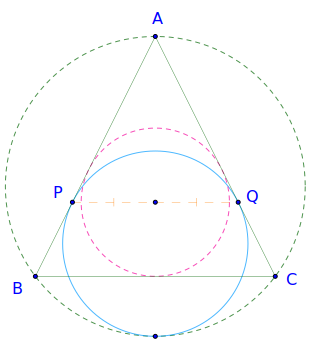
\includegraphics[width=4cm]{./svg/pdf/homothety-p6a.pdf}
    \end{center}
\end{frame}

\begin{frame}[t]
    \frametitle{Geometric Transformations IV}
    \framesubtitle{Homothety - Example 6}
    \begin{overprint}
        \onslide<1>Let $E$ be the center of the circle $\omega$, which is tangent with $AB$, $AC$, and $(ABC)$.
        Let $D$ be the tangent point of the two circles, $M$ be the midpoint of $BC$, and $F$ be the midpoint of $PQ$.
        It is easy to see that $A,F,E,M,D$ are collinear.
        Let $\mathcal{H}_{(A,k)}$ be a homothety centred at $A$ and $\mathcal{H}_{(A,k)}(D)=M.$
        Since $AF/AM = AE/AD$, so $\mathcal{H}_{(A,k)}(E)=F.$
        \begin{center}
            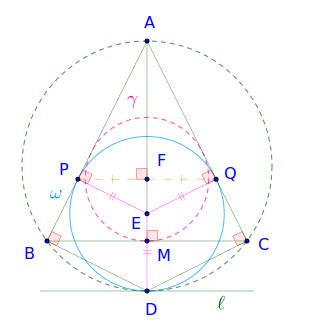
\includegraphics[width=5cm]{./svg/pdf/homothety-p6b.pdf}
        \end{center}
        \onslide<2>Let $\gamma$ be the image of $\omega$, $\gamma=\mathcal{H}_{(A,k)}(\omega).$
        Since $\omega$ is tangent $(ABC)$ at $D$, so both are tangent with line $\ell$ through $D$ parallel with $BC,$
        thus $\gamma$ tangent with the image of $\ell$, which is line $BC$.
        Furthermore, the $\mathcal{H}_{(A,k)}(D)=M,$ keeps $B$ and $C$ on rays $AB$ and $AC$, and because $\omega$ is tangent to $AB$ and $AC$,
        so $\gamma$ is also tangent to $AB$ and $AC$.        
        \begin{center}
            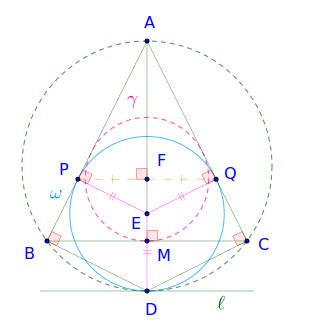
\includegraphics[width=5cm]{./svg/pdf/homothety-p6b.pdf}
        \end{center}
        \onslide<3>Therefore $\gamma$ is tangent with all sides of $\triangle ABC$, so $\gamma = I_{\triangle ABC}.$

        Therefore, the image of $\mathcal{H}_{(A,k)}(E)$ is $I$, the incentre of $\triangle ABC$, therefore $F \equiv I.$

        Hence, \framebox{the midpoint of $PQ$ is the center of the inscribed circle of the triangle $ABC.$}
        \begin{center}
            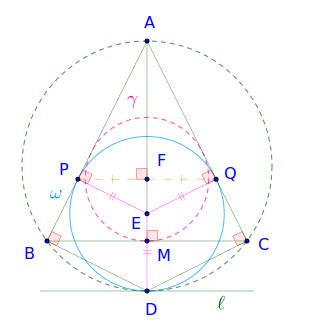
\includegraphics[width=5cm]{./svg/pdf/homothety-p6b.pdf}
        \end{center}
    \end{overprint}
\end{frame}

\begin{frame}[t]
    \frametitle{Geometric Transformations IV}
    \framesubtitle{Homothety - Example 7}
    \begin{example}
        Three congruent circles have a common point $P$ and lie inside a given triangle. Each circle touches a pair of sides of the triangle.
        \bigbreak
        Prove that the incenter and the circumcenter of the triangle and the point $P$ are collinear.
    \end{example}
    \begin{center}
        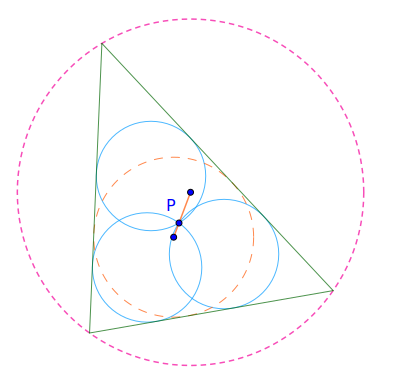
\includegraphics[width=5cm]{./svg/pdf/homothety-p7a.pdf}
    \end{center}
\end{frame}

\begin{frame}[t]
    \frametitle{Geometric Transformations IV}
    \framesubtitle{Homothety - Example 7}
    Let $A'$, $B'$, $C'$ be the centers of the circles. Since the radii are the same, so $A'B'$ is parallel to $AB$, $B'C'$ is parallel to $BC$, $C'A'$ is parallel to $CA$.
    Since $AA'$, $BB'$, $CC'$ bisect $\angle A$, $\angle B$, $\angle C$, respectively, they concur at the incenter $I$ of $\triangle ABC.$
    \begin{center}
        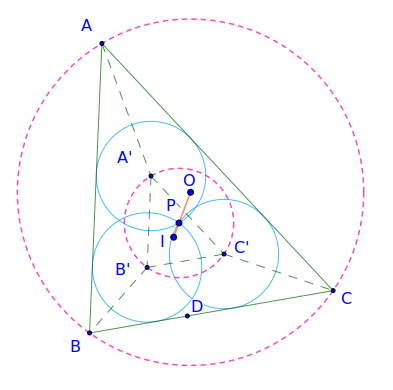
\includegraphics[width=5cm]{./svg/pdf/homothety-p7b.pdf}
    \end{center}
    Note $P$is the circumcenter of $\triangle A'B'C'$ as it is equidistant from $A', B', C'$.
    Then the homothety with center $I$ sending $\triangle A'B'C'$ to $\triangle ABC$ will send $O$ to the circumcenter $O$ of $\triangle ABC.$
    Therefore, $I, P, O$ are collinear.
\end{frame}

\begin{frame}[t]
    \frametitle{Geometric Transformations IV}
    \framesubtitle{Homothety - Example 8}
    \begin{example}
        A non-isosceles triangle $A_{1}A_{2}A_{3}$ has sides $a_{1}$, $a_{2}$, $a_{3}$
        with the side $a_{i}$ lying opposite to the vertex $A_{i}$.
        Let $M_{i}$ be the midpoint of the side $a_{i}$,
        and let $T_{i}$ be the point
        where the inscribed circle of triangle $A_{1}A_{2}A_{3}$ touches the side $a_{i}$.
        Denote by $S_{i}$ the reflection of the point $T_{i}$
        in the interior angle bisector of the angle $A_{i}$.
        \bigbreak
        Prove that the lines $M_{1}S_{1}$, $M_{2}S_{2}$ and $M_{3}S_{3}$ are concurrent.
    \end{example}
    \begin{center}
        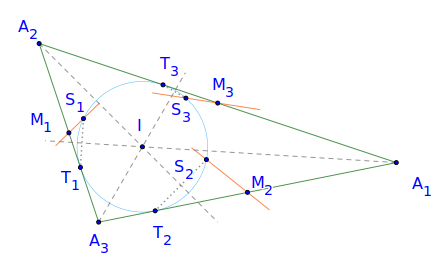
\includegraphics[width=6cm]{./svg/pdf/homothety-p8a.pdf}
    \end{center}
\end{frame}

\begin{frame}[t]
    \frametitle{Geometric Transformations IV}
    \framesubtitle{Homothety - Example 8}
    \begin{overprint}
        \onslide<1>Let $I$ be the incenter of $\triangle A_1A_2A_3.$ Let $B_1$, $B_2$, $B_3$ be the points where the internal angle bisectors of $\angle A_1$, $\angle A_2$, and $\angle A_3$
        meet sides $a_1$, $a_2$, $a_3$ respectively.

        \bigbreak
        With respect to $A_1B_1$, the reflection of $T_1$ is $S_1$ and the reflection of $T_2$ is $T_3$. So $\angle T_3IS_1 = \angle T_2IT_1.$
        
        With respect to $A_2B_2$, the reflection of $T_2$ is $S_2$ and the reflection of $T_1$ is $S_3.$ So $\angle T_3IS_2 = \angle T_1IT_2.$

        Then $\angle T_3IS_1 = \angle T_3IS_2.$
        \begin{center}
            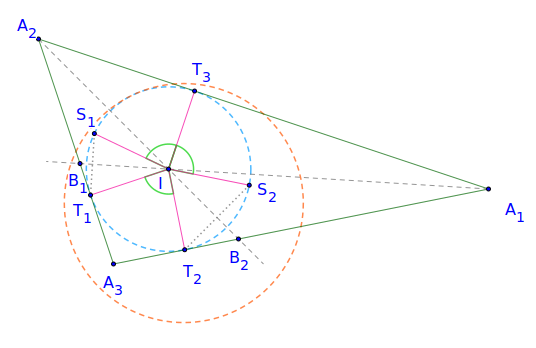
\includegraphics[width=6cm]{./svg/pdf/homothety-p8b.pdf}
        \end{center}
        \onslide<2>Since $IT_3$ is perpendicular to $A_1A_2$, we get $S_2S_1$ is parallel to $A_1A_2$.
        
        Since $A_1A_2$ is parallel to $M_2M_1$, we get $S_2S_1$ is parallel to $M_2M_1.$
        
        Similarly, $S_3S_2$ is parallel to $M_3M_2$ and $S_1S_3$ is parallel to $M_1M_3.$
        \bigbreak
        Thus the sides of $\triangle S_1S_2S_3$ and $\triangle M_1M_2M_3$ are pairwise parallel.
        \begin{center}
            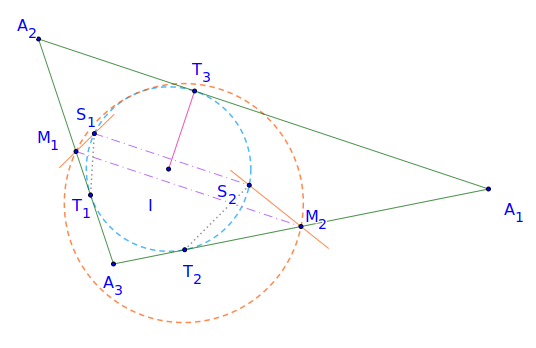
\includegraphics[width=6cm]{./svg/pdf/homothety-p8d.pdf}
        \end{center}
        \onslide<3>Now the circumcircle of $\triangle S_1S_2S_3$ is the incircle of $\triangle A_1A_2A_3$ 
        and the circumcircle of $\triangle M_1M_2M_3$ is the nine point circle of $\triangle A_1A_2A_3$.
        \bigbreak
        Since $\triangle A_1A_2A_3$ is not equilateral, these circles have different radii (why?).
        \bigbreak
        Hence $\triangle S_1S_2S_3$ is not congruent to $\triangle M_1M_2M_3$, and because their sides are pairwise parallel,
        thus there is a homothety sending $\triangle S_1S_2S_3$ to $\triangle M_1M_2M_3$ (why?)
        \bigbreak
        Then $M_1S_1, M_2S_2$. and $M_3S_3$ concur at the center of the homothety.
        \begin{center}
            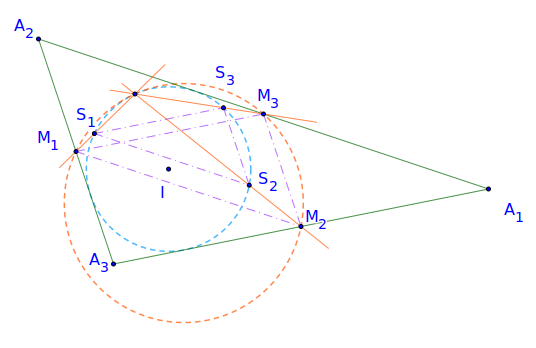
\includegraphics[width=6cm]{./svg/pdf/homothety-p8c.pdf}
        \end{center}
    \end{overprint}
\end{frame}

\begin{frame}[t]
    \frametitle{Geometric Transformations IV}
    \framesubtitle{Homothety - Example 9}
    \begin{example}
        Two weather buoy float near the shore at points $A$ and $B$.
        How can you draw a line through a point $M$ on the shore parallel to $AB$?
    \end{example}
    \begin{center}
        \includegraphics[width=3cm]{./png/NOAA-NDBC-discus-buoy.jpg}
        \qquad
        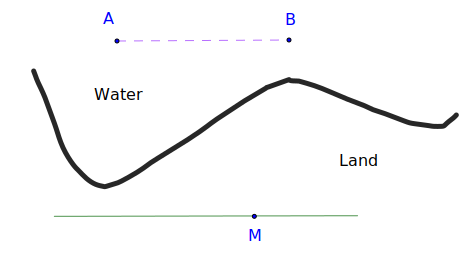
\includegraphics[width=7cm]{./svg/pdf/homothety-p9.pdf}
    \end{center}
\end{frame}

\end{document}

